\section{Fennel}
\label{sec:fennel}

\begin{spice}\label{spice:fennel}
\textsc{Fennel} \hfill \href{https://powo.science.kew.org/taxon/842680-1}{POWO} \\
\textbf{English:} \textit{fennel}. 
\textbf{Arabic:} {\arabicfont{شمر}} \textit{shamar}. 
\textbf{Chinese:} {\traditionalchinesefont{茴香}} \textit{huíxiāng} [hui-spice]; \traditionalchinesefont{小茴香} \textit{xiǎohúixiāng} [little-hui-spice]. 
\textbf{Hungarian:} \textit{édeskömény} [sweet-cumin]; \textit{ánizskapor} [anise-dill].  \\
\noindent{\color{black}\rule[0.5ex]{\linewidth}{.5pt}}
\begin{tabular}{@{}p{0.25\linewidth}@{}p{0.75\linewidth}@{}}
Plant species: & \taxonn{Foeniculum vulgare}{Mill.} \\
Family: & \textit{Apiaceae} \\
part used: & fruit; leaf \\
Region of origin: & Med \\
Cultivated in: & Argentina; Bulgaria; Germany; Greece; India; Lebanon \\
Color: & light green to light brown \\
\end{tabular}
\end{spice}

\begin{figure}[!ht]
	\vspace{-4ex}
	\centering
	\subfloat[\centering a]{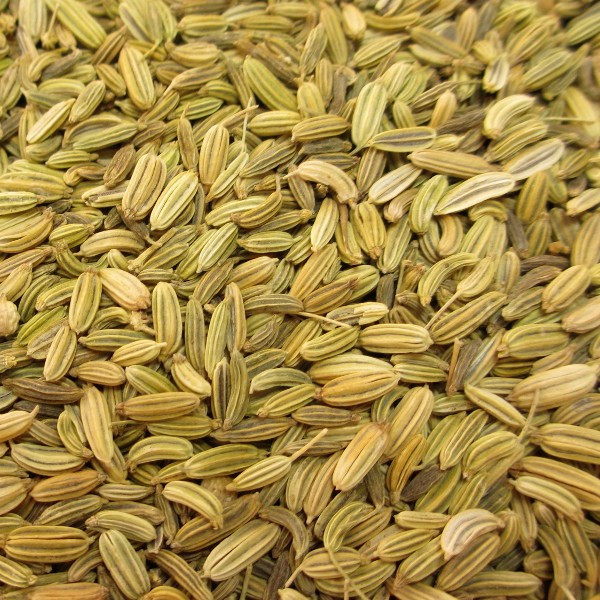
\includegraphics[width=0.3\linewidth]{imgs/spices/fennel-1.jpg}}
% 	\hfill
% 	\subfloat[\centering b]{\includegraphics[width=0.3\linewidth]{imgs/spices/fennel-2.jpg}}
% 	\hfill
% 	\subfloat[\centering c]{\includegraphics[width=0.3\linewidth]{imgs/spices/fennel-3.jpg}}
	\caption{Fennel \taxon{}.}
	\label{fig:fennel_imgs}
\end{figure}

\subsection{The Botany of Fennel}

\subsection{The History of Fennel}

\subsection{The Names of Fennel}

\subsubsection{English}

\begin{etymology}\label{ety:fennel}
\textbf{English} \textit{fennel}, a. 700
< \textbf{Old English} \textit{fenol}, a. 700
< \textbf{Latin} \textit{faeniculum}, via Vulgar Latin \textit{fēnoclum, fēnuclum} substituted for classical Latin \textit{faeniculum}, diminutive of \textit{faenum} hay; cf. Old French fenoil (modern French fenouil), Provençal fenolh, Italian finocchio, Spanish hinojo.\footnote{\textcite[s.v. fennel]{oed}; }
\end{etymology}

\begin{table}[!ht]
\centering
\begin{tabularx}{\textwidth}{@{}l>{\itshape \small}lL>{\small}l@{}}
\toprule
\textbf{\#} & \multicolumn{1}{l}{\textbf{Species}} & \multicolumn{1}{l}{\textbf{Name}} & \multicolumn{1}{l}{\textbf{Source}} \\
\midrule
\textbf{1}	& \textbf{Foeniculum vulgare}	& \textbf{fennel}	& \textbf{\textcite{van_wyk_culinary_2014}} \\
2	& Foeniculum vulgare	& fennel-seed	& \textcite{oed} \\
3	& Foeniculum vulgare	& Indian fennel	& \textcite{van_wyk_culinary_2014} \\
4	& Foeniculum vulgare	& sweet fennel	& \textcite{van_wyk_culinary_2014} \\
\bottomrule
\end{tabularx}
\caption{Various names for fennel in English.}
\label{table:names_fennel_en}
\end{table}



\subsubsection{Arabic}

\begin{table}[!ht]
\centering
\begin{tabularx}{\textwidth}{@{}l>{\itshape \small}lr>{\itshape}lL>{\small}l@{}}
\toprule
\textbf{\#} & \multicolumn{1}{l}{\textbf{Species}} & \multicolumn{1}{l}{\textbf{Name}} & \multicolumn{1}{l}{\textbf{Tr.}} & \multicolumn{1}{l}{\textbf{Gloss}} & \multicolumn{1}{l}{\textbf{Source}} \\
\midrule
1	& Foeniculum vulgare	& بسباس	& basbās	& 	& \textcite{wehr_dictionary_1976} \\
2	& Foeniculum vulgare	& رازيانج 	& rāzyānj	& 	&  \\
\textbf{3}	& \textbf{Foeniculum vulgare}	& \textbf{ شمر}	& \textbf{shamar}	& \textbf{}	& \textbf{\textcite{wehr_dictionary_1976}} \\
4	& Foeniculum vulgare	& شمرة	& shamra, shumra	& 	& \textcite{wehr_dictionary_1976} \\
5	& Foeniculum vulgare	&  شمار	& shamār	& 	& \textcite{wehr_dictionary_1976} \\
6	& Foeniculum vulgare	& سنوت	& sunūt	& 	&  \\
\bottomrule
\end{tabularx}
\caption{Various names for fennel in Arabic.}
\label{table:names_fennel_ar}
\end{table}



\subsubsection{Chinese}

\begin{table}[!ht]
    \caption{Various names for fennel in Chinese.}
\centering
\begin{tabularx}{\textwidth}{@{}l>{\itshape \small}ll>{\itshape}lL>{\small}l@{}}
\toprule
\textbf{\#} & \multicolumn{1}{l}{\textbf{Species}} & \multicolumn{1}{l}{\textbf{Name}} & \multicolumn{1}{l}{\textbf{Tr.}} & \multicolumn{1}{l}{\textbf{Gloss}} & \multicolumn{1}{l}{\textbf{Source}} \\
\midrule
1	& Foeniculum vulgare	& \tc{蘹香}	& huáixiāng	& huai-spice	&  \\
\textbf{2}	& \textbf{Foeniculum vulgare}	& \textbf{\tc{茴香}}	& \textbf{huíxiāng}	& \textbf{hui-spice}	& \textbf{\textcite{kleeman_oxford_2010}} \\
3	& Foeniculum vulgare	& \tc{甜茴香}	& tiánhuíxiāng	& sweet-fennel	&  \\
4	& Foeniculum vulgare	& \tc{小茴香}	& xiǎohuíxiāng	& small-anise	&  \\
\bottomrule
\end{tabularx}
\label{table:names_fennel_zh}
\end{table}



\subsubsection{Summary}

\begin{table}[!ht]
    \caption{Conventionalized names for fennel in English, Arabic, and Chinese, found in dictionaries.}
\centering
\begin{tabularx}{\textwidth}{@{}ll>{\itshape}lLl>{\small}l@{}}
\toprule
\textbf{\#} & \textbf{Language} & \multicolumn{1}{l}{\textbf{Term}} & \textbf{Gloss} & \textbf{Loan} & \multicolumn{1}{l}{\textbf{Source}} \\
\midrule
1	& English	& fennel	& 	& yes	& \textcite{oed} \\
2	& English	& fennel-seed	& 	& no	& \textcite{oed} \\
3	& English	& Indian fennel	& 	& no	& \textcite{oed} \\
4	& English	& sweet fennel	& 	& no	& \textcite{oed} \\
\midrule
1	& Arabic	& basbās	& 	& yes	& \textcite{wehr_dictionary_1976} \\
2	& Arabic	& shamar	& 	& yes	& \textcite{wehr_dictionary_1976} \\
3	& Arabic	& shamra, shumra	& 	& yes	& \textcite{wehr_dictionary_1976} \\
4	& Arabic	& shamār	& 	& yes	& \textcite{wehr_dictionary_1976} \\
\midrule
1	& Chinese	& huíxiāng	& hui-spice	& no	& \textcite{kleeman_oxford_2010} \\
\bottomrule
\end{tabularx}
\label{table:names_fennel}
\end{table}

